% Circular arrows with text
% Author: Tom Bombadil
\documentclass[tikz,border=10pt]{standalone}
%%%<
\usepackage{verbatim}
\usepackage{xcolor}
\definecolor{BH}{HTML}{97004D}
%%%>
\begin{comment}
:Title: Circular arrows with text
:Tags: Arrows;Decorations;Arcs;Foreach;Diagrams
:Author: Tom Bombadil
:Slug: circular-arrows-text

This example was written by Tom Bombadil answering a question on TeX.SE,
with a modification by Stefan Kottwitz adding a text font style
showing an implicit way.
\end{comment}
\usetikzlibrary{decorations.text}
\newcommand*{\mytextstyle}{\sffamily\Large\bfseries\color{black!85}}
\newcommand{\arcarrow}[8]{%
% inner radius, middle radius, outer radius, start angle,
% end angle, tip protusion angle, options, text
  \pgfmathsetmacro{\rin}{#1}
  \pgfmathsetmacro{\rmid}{#2}
  \pgfmathsetmacro{\rout}{#3}
  \pgfmathsetmacro{\astart}{#4}
  \pgfmathsetmacro{\aend}{#5}
  \pgfmathsetmacro{\atip}{#6}
  \fill[#7] (\astart:\rin) arc (\astart:\aend:\rin)
       -- (\aend+\atip:\rmid) -- (\aend:\rout) arc (\aend:\astart:\rout)
       -- (\astart+\atip:\rmid) -- cycle;
  \path[font = \sffamily, decoration = {text along path, text = {|\mytextstyle|#8},
    text align = {align = center}, raise = -0.5ex}, decorate]
    (\astart+\atip:\rmid) arc (\astart+\atip:\aend+\atip:\rmid);
}

\begin{document}
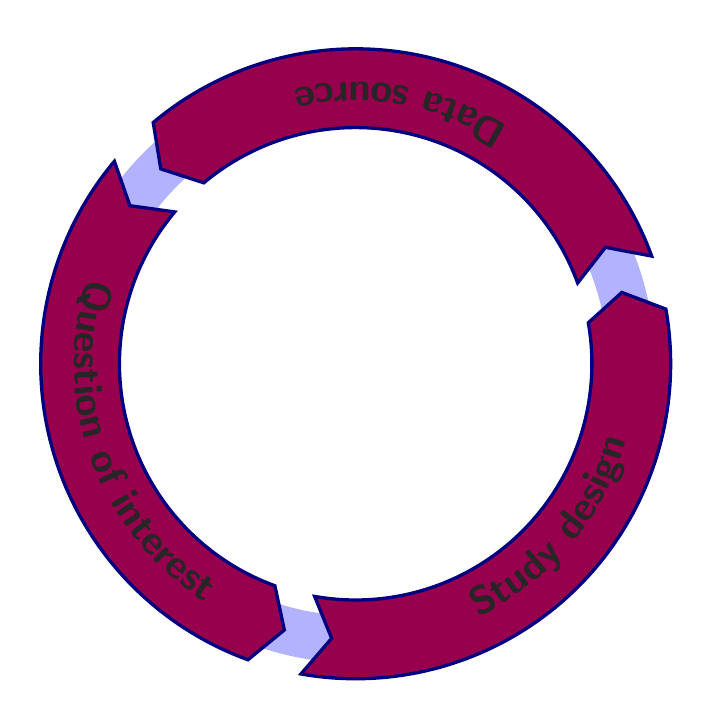
\begin{tikzpicture}
  \fill[even odd rule,blue!30] circle (3.8) circle (3.2);
  \arcarrow{3}{3.5}{4}{20}{130}{5}{BH,
    draw = blue!50!black, very thick}{Data source}
  \arcarrow{3}{3.5}{4}{140}{250}{5}{BH,
    draw = blue!50!black, very thick}{Question of interest}
  \arcarrow{3}{3.5}{4}{260}{370}{5}{BH,
    draw = blue!50!black, very thick}{Study design}
\end{tikzpicture}
\end{document}

%%% Local Variables: 
%%% mode: latex
%%% TeX-master: t
%%% End: 
